\section{Realizacja poszczególnych elementów systemu}
\subsection{Realizacja warstwy genetycznej}
\subsubsection{Struktura danych chromosomu}
\begin{par}
	Jeśli chodzi o typ struktury danych przyjęto pierwszy schemat (rys.\ref{fig:sterowanie}), wraz z krzyżowaniem statystycznym. 
	O ile ukierunkowanie systemu na gry jednego typu może lepiej się sprawdzić jeśli zależy nam
	jedynie na szybkim i optymalnym wyniku, to generalizacja systemu i elastyczna implementacja całego algorytmu da nam lepsze narzędzie nie tylko dydaktyczne, ale też badawcze.
	Przykładem może być popularna gra Galaxian. Sama definicja klawiszy w Galaxian i Super Mario Brothers jest podobna (klawisze kierunkowe + klawisze specjalne),
	jednak schemat poruszania się jest już inny: O ile gry typu Mario Brothers pasują do powyższych założeń o kierunkowości ruchu, to w grze Galaxian już tak nie jest.
	Korzystniej zatem jest traktowanie projektu jako systemu rozwiązującego gry platformowe czasu rzeczywistego na podstawie przyciśnięć klawiszy w czasie.
\end{par}
\begin{par}
	
	Sam chromosom przechowuje następujące dane:

	\begin{itemize}
		\item Tablicę dotyczącą akcji ruchu przechowującą wartości typu wyliczeniowego: UP, DOWN, LEFT, RIGHT, NONE
		\item Tablicę dotyczącą akcji specjalnych: A, B, C, D, NONE
		\item Instancję obiektu \textit{ResultData} przechowującego dane dotyczące wyniku funkcji przystosowania, oraz wartości ustalane po przetestowaniu danego chromosomu takie jak czas który upłynął, rodzaj wyniku, ilość zebranych punktów.
	\end{itemize}

	Wartość NONE w obu tablicach odpowiada za brak akcji. 
	Wartości A,B,C,D odpowiadają za kolejne klawisze specjalne które mogą być traktowane przez środowisko gry jako skok lub strzał. 
	Ograniczamy się do 4 klawiszy specjalnych, które wystarczają w zupełności do zrealizowania większości gier platformowych.

	Oprócz tego każdy Chromosom uzupełnia interfejs Comparable, dzięki czemu obiekty mogą być porównywane ze sobą. Porównanie składa się jedynie z porównania wyniku wartości funkcji przystosowania. Dzięki temu możemy łatwo posortować całe populacje.
	Obiekt ten przechowuje dane na temat wyniku danego chromosomu i danych pomocniczych, które sa uzupełniane po przetestowaniu chromosomu. 
	Oprócz tego chromosom posiada metody pozwalające na mutację zarówno tablicy ruchu jak i tablicy akcji specjalnych.
\end{par}
\subsubsection{Dane konfiguracyjne}
\begin{par}
	Jak już zostało wspomniane, podstawą dobrego systemu, szczególnie do zastosowań badawczych jest łatwo dostępna konfiguracja. 
	W pracy rolę tę pełni pośrednio klasa \textit{GeneticsConfig} która zawiera wszystkie najważniejsze parametry dotyczące algorytmu (takie jak prawdopodobieństwo mutacji) są przechowywane jako wartości tablicy asocjacyjnej (klasa \textit{JHashMap}). 
	Oprócz tego sama tablica została opakowana w taki sposób iż rejestracja nowej wartości do tablicy wiąże się z automatycznym wygenerowaniem odpowiedniego pola w panelu konfiguracyjnym. 
	Dzięki temu mamy pewność iż wszystkie parametry biorące udział w algorytmie będą w pełni konfigurowalne.
\end{par}
\begin{par}
	Każda z akcji, zarówno ruchu jak i specjalna posiada prawdopodobieństwo wystąpienia.
	Wartości te również dostępne są w panelu konfiguracyjnym, przy czym są one normalizowane do sumy wszystkich wartości z danej kategorii.
	Przykładowo dla wartości podanych na rys \ref{fig:config1}. Wartość ruchu w prawo (grupa ``Movement key probabilities'') wynosi $\frac{2.5}{2.5+0.5+0.2}=0.78125$.
	\begin{figure}[!h]
		\centering
		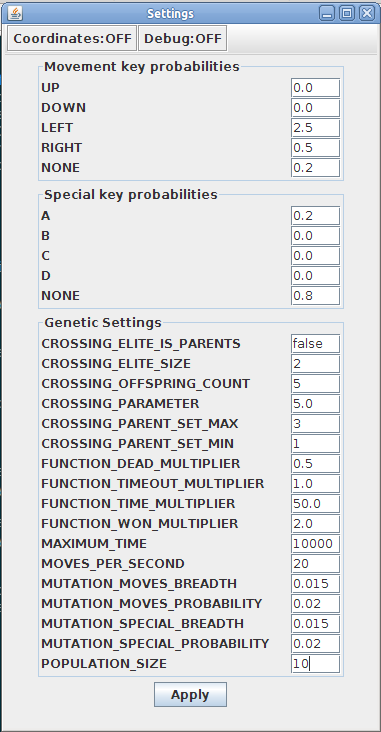
\includegraphics[width=2in]{obrazki/config1.png}
		\caption{Panel Konfiguracyjny.}
		\label{fig:config1}
	\end{figure}
	Oprócz tego klasa GeneticsConfig posiada metody pozwalające na zwrócenie losowej akcji w zależności od prawdopodobieństwa jej wystąpienia - Rys. \ref{fig:config1}.
\end{par}
\subsubsection{Widok Populacji i Chromosomu}
\begin{par}

	\begin{figure}[!h]
		\centering
		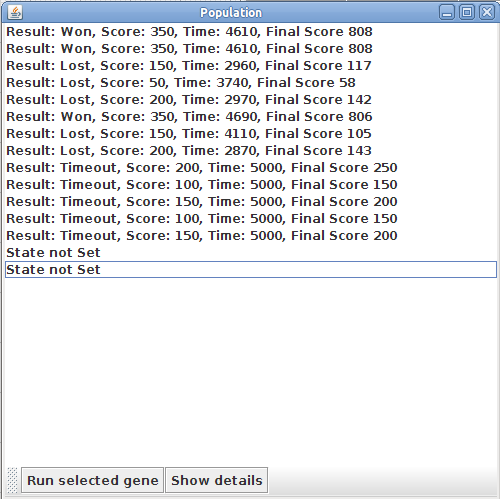
\includegraphics[width=4in]{obrazki/populacja.png}
		\caption{Okno populacji.}
		\label{fig:populacja}
	\end{figure}


	\begin{figure}[!h]
		\centering
		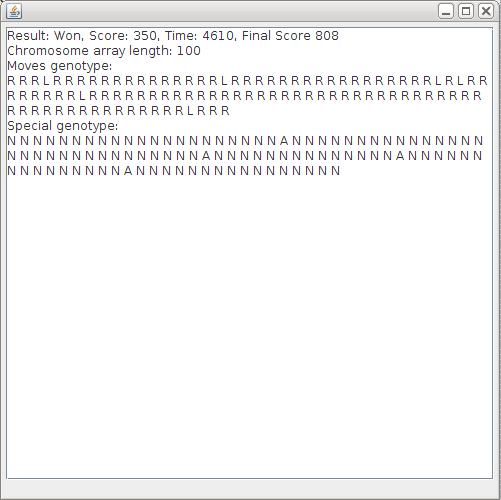
\includegraphics[width=4in]{obrazki/chromosom.png}
		\caption{Okno szczegółów chromosomu.}
		\label{fig:chromosom}
	\end{figure}
\end{par}




\subsection{Realizacja warstwy symulacyjnej}
\subsubsection{Logika gry}
\begin{par}
	Sama warstwa logiki gry podejmuje decyzje o relacjach pomiędzy obiektami w grze.
	Wszystkie elementy gry dziedziczą po klasie \textit{WorldObject}, która przechowuje podstawowe dane konieczne do wyświetlenia go w oknie takie jak położenie oraz wymiary.
	Kolejno można je podzielić na:
	\begin{itemize}
		\item Obiekt klasy \textit{Actor}. 
		Obiekt reprezentujący postać w grze. 
		Klasa ta posiada zmienną \textit{velocity}, oznaczającą wektor prędkości obiektu.  
		W każdym cyklu gry zostaje on dodany do położenia aktora.
		Na zmianę wektora wpływa klasa \textit{Controller} która w zależności od trybu gry przekazuje wciśnięcia klawiszy z klawiatury, lub akcje wygenerowane przez algorytm genetyczny.
		\item Obiekt klasy \textit{Terrain}. Z nich zbudowana jest mapa gry. Z punktu widzenia logiki nie wpływają one w żaden sposób na wynik, a jedynie kolidują z obiektem aktora. To z nich zbudowana jest mapa gry.
		\item Obiekty klasy \textit{Bonus}
		Są to obiekty wpływające na wynik gry. Kolizja Aktora z nimi powoduje zmianę wyniku gry. Klasa \textit{Bonus} jest klasą po której dziedziczą podklasy:
		\begin{itemize}
			\item BonusCoin - Obiekt reprezentujący punkty w grze. Aktorowi po kolizji z nimi zostaje dodana wartość punktowa przechowywana w obiekcie. Z punktu widzenia algorytmu zwiększają one ostateczną wartość funkcji przystosowania, która zależy od ilości punktów zebranych na mapie.
			\item BonusWin - Kolizja aktora z obiektem tego typu kończy przejście chromosomu bądź gracza i zapisuje w stanie gry wynik końcowy \textit{RESULT\_WON}. W praktyce oznacza on zakończenie gry z pozytywnym skutkiem, który jest brany pod uwagę podczas wyliczenia funkcji przystosowania.
			\item BonusLose - Obiekt kończący grę ze skutkiem negatywnym. Ma on reprezentować wszelkiego rodzaju pułapki w grze, które natychmiastowo kończą przejście chromosomu. W stanie gry zostaje wówczas zapisany wynik końcowy \textit{RESULT\_LOST}.
		\end{itemize}
	\end{itemize}
	\definecolor{orange}{rgb}{1,0.5,0}
	\definecolor{gray}{rgb}{0.5,0.5,0.5}
	Na Rys. \ref{fig:objects} widać obiekty świata gry: 
	\textcolor{blue}{\textit{Actor}}, 
	\textcolor{orange}{\textit{BonusCoin}},
	\textcolor{red}{\textit{BonusLose}},
	\textcolor{green}{\textit{BonusWin}},
	\textcolor{black}{\textit{Terrain}}.

	\begin{figure}[!h]
		\centering
		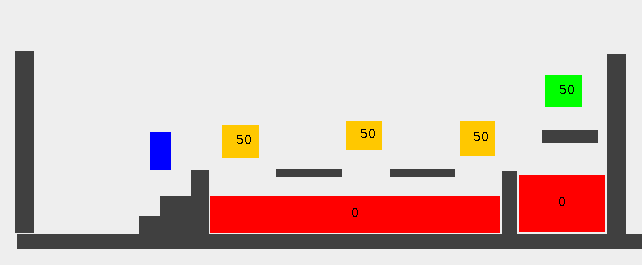
\includegraphics[width=4in]{obrazki/objects.png}
		\caption{Poszczególne elementy mapy.}
		\label{fig:objects}
	\end{figure}
\end{par}

\begin{par}
	Podstawową logiką gry i detekcją kolizji pomiędzy obiektami zarządza obiekt klasy \textit{Logic}. Użytym w pracy schematem logiki jest schemat gry ``Super Mario Brothers''. Wobec czego domyślną logiką gry przy uruchomieniu programu jest instankcja klasy \textit{LogicMario}
	Zakłada ona ruch w 2 kierunkach, skok oraz działanie grawitacji na obiekt aktora.
	Ponieważ klasa \textit{LogicMario} dziedziczy po klasie \textit{Logic} możliwe jest napisanie własnej logiki i podmiana tej obowiązującej w systemie.
	Ponieważ działanie algorytmu nie jest związane z fizyką ani zasadami obowiązującymi w grze, system może działać dla wielu różnych typów gier platformowych i zręcznościowych.
	Jedynym wymogiem jest to iż muszą one dać się opisać za pomocą wyżej zdefiniowanych klas i cech:
	\begin{enumerate}
		\item
			Obiekty świata muszą należeć do którejś z klas dziedziczących po klasie \textit{WorldObject}.
		\item 
			Możliwe rezultaty zakończenia algorytmu muszą być wśród zbioru rezultatów: \{Koniec Czasu, Wygrana, Przegrana\}, 
		\item
			Rodzaje możliwych akcji do wykonania w grze muszą być przypisane do 4 akcji ruchu kierunkowego oraz 4 akcji specjalnych.
	\end{enumerate}

	Jedyną pracą jaką należy wykonać przy implementacji własnego środowiska gry jest uzupełnienie własnej klasy dziedziczącej po klasie \textit{Logic}.
	Wówczas przy poprawnej implementacji logiki gry system automatycznie symuluje zbiory chromosomów w środowisku gry.
\end{par}
\subsubsection{Edytor Map}
\begin{par}
Przy testowaniu różnych ustawień algorytmu genetycznego przydatnym narzędziem może okazać się edytor map. 
Ustawienia algorytmu, szczególnie dotyczące prawdopodobieństwa wylosowania akcji w dużej mierze zależą od typu mapy. 
\begin{itemize}
\item 
Mapa może być ukierunkowana bądź nie, wówczas ustawienie odpowiedniego stosunku akcji ruchu może znacznie przyspieszyć szukanie wyniku. Przykładowo: Jeśli problemem jest znalezienie rozwiązania na szerokiej mapie, której cel znajduje się w jej prawym krańcu, dobrą strategią będzie ustawienie ruchu w prawo na wysoką wartość np. $0.95$ a ruchu w lewo na wartość $0.05$.
\item
Podobna sytuacja ma miejsce z akcjami specjalnymi. 
Należy pamiętać iż wartość \textit{NONE} może być szczególnie istotna w ustawieniach genetycznych akcji specjalnych.
Powołując się znów na przykład gry ``Super Mario Brothers'', można zauważyć iż ciągły skok nie koniecznie jest optymalną strategią - przez większość czasu nasza postać porusza się po podłożu.
\item 
Logika gry może zakładać różną ilość kierunków w których można się poruszać, co w dużej mierze zależy od typu gry jaki reprezentuje.
Niektóre wymagają 2 klawiszy kierunkowych do poruszania się po mapie, inne 3 lub 4. 
Aby nie brać pod uwagę akcji które i tak nie będa interpretowane przez logikę, najlepiej jest ustalić prawdopodobieństwo wylosowania ruchów nieaktywnych na wartość $0$. 
Wówczas istnieje pewność iż w genotypie nie znajdują się niepotrzebne informacje.
\end{itemize}

Dobrze zaprojektowany edytor map może okazać się szczególnie przydatny dla bardziej zaawansowanych użytkowników którzy mogą korzystać z systemu w celach edukacyjnych, a logiki zaimplementowane w systemie nie spełniają ich wszystkich oczekiwań.
Wówczas po napisaniu własnej klasy odpowiadajacej za logikę, dobrze jest skonstruować mapy odpowiadające typowi rozgrywki jakie logika przewiduje.

\begin{par}
	Po otworzeniu edytora map domyślnie wczytywana jest bieżąca mapa, dzięki czemu można dokonać szybkich edycji jeśli koniecznie jest sprawdzenie działania algorytmu z pewnym wariantem, lub dodatkowym obiektem na mapie.
	Oprócz tego wszystkie mapy zapisywane są w prostym formacie tekstowym, dzięki czemu możliwe jest generowanie map przy pomocy programów trzecich, lub skryptów - zostawia to bardziej zainteresowanym użytkownikom na generowanie dużych, losowych poziomów, o ile wcześniej zaznajomią się z formatem zapisu mapy.
	Przykładowy plik z mapą może wyglądać następująco:
	
	\begin{lstlisting}
		Terrain 122 361 239 27
		Terrain 110 211 25 151
		Terrain 355 201 28 165
		Actor 140 295 20 32
		BonusCoin 202 328 18 30 25
		BonusCoin 248 330 16 27 25
		BonusWin 327 236 18 36 25
		BonusLose 313 311 33 40 0
	\end{lstlisting}

	Pierwszym elementem każdego wiersza jest nazwa klasy.
	Kolejne wartości to punkt oznaczający położenie lewego górnego rogu obiektu, oraz jego szerokość i wysokość.
	W wypadku obiektów klasy \textit{Bonus} ostatnia liczba oznacza wartość punktową. 
	Zachowanie prostego formatu mapy uprościło proces sprawdzania aplikacji, oraz otworzyło możliwość generowania dużych map poprzez skrypty.
	Ponieważ nie było powodu aby przechowywać mapy jako dane binarne - samo wczytywanie mapy nie spowalnia aplikacji, nie jest wykonywane często - otwarty format pozostał jako obowiązujący w systemie.
\end{par}

		\begin{figure}[!h]
		\centering
		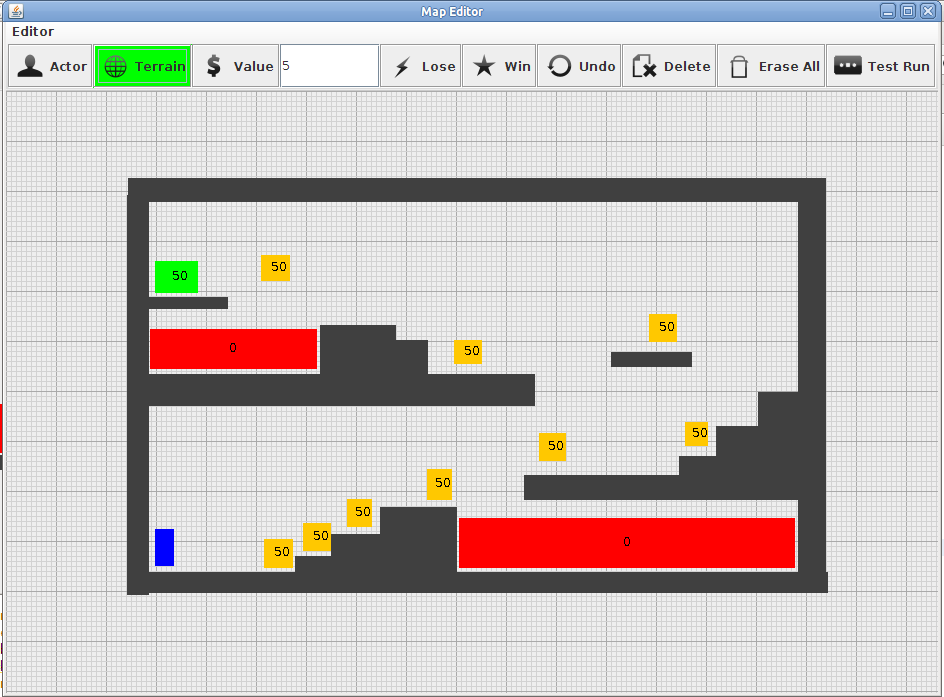
\includegraphics[width=4in]{obrazki/map_editor.png}
		\caption{Okno edytora map.}
		\label{fig:map_editor}
	\end{figure}
\end{par}




\subsection{Użyte narzędzia i technologie}
\begin{par}
	\subsection{Język aplikacji}
	System został napisany w języku Java oraz testowany na wirtualnej maszynie javy w wersji Java SE 7u2. Biblioteka Swing została użyta do stworzenia warstwy wizualnej programu.
	\subsection{Java}
	Java jest językiem programowania wysokiego poziomu zaprojektowanym i stworzonym przez Jamesa Groslinga podczas gry pracował w firmie Sun Microsystems. Pierwsza propozycja stworzenia Javy pojawiłą się w roku 1991, do głównych twórców oprócz Jamesa Groslinga zalicza się również Mike'a Sheridana oraz Patrick'a Naughtona.
	Początkowo język Java był bezpośrednio związany z firmą Sun Microsystems, która kontrolowała jego rozwój do roku 2010.
	Od tego czasu firma Sun stała się częścią korporacji Oracle, wobec czego wszelkie prawa związane z językiem Java posiada Oracle.
	Java swoją składnią przypomina język C, aczkolwiek wśród pierwowzorów wymienia się również język Smalltalk.
	Aplikacje napisane w języku Java są kompilowane do kodu bajtowego Javy (ang. java bytecode), i uruchamiane na maszynie wirtualnej, co zapewnia pewnego rodzaju bezpieczeństwo w stosunku do języka C lub C++.
	Inną dużą zaletą języka Java jest jego przenośność.
	Jedynym wymogiem uruchomienia aplikacji javowej na dowolnym systemie jest obecność wirtualnej maszyny javy (ang. JVM - Java Virtual Machine).
	Dziś większość urządzeń mobilnych posiada maszynę wirtualną javy pozwalającą na uruchamianie aplikacji napisanych w tymże języku.
	::BIBLIOGRAFIA TIJ-Bruce Eckel::
	Jak pisze Bruce Eckel w swojej ksiażce poświęconej językowi Java: ``To, co wywarło na mnie największe wrażenie, kiedy poznawałem javę, to fakt, że wśród innych celów projektantów z firmy Sun znalazła się także redukcja złożoności dla programisty. 
	To tak, jakby powiedzieć: ``Nie dbamy o nic poza zmniejszeniem czasu i trudności tworzenia porządnego kodu.''(...)''
	Po kilku latach styczności z językiem, trudno jest się nie zgodzić z powyższym stwierdzeniem.
	\subsection{Swing}
	Pierwszą próbą stworzenia biblioteki pozwalającej na tworzenie graficznego interfejsu użytkownika była biblioteka AWT (ang. Abstract Window Toolkit).
	Fala niezawodolenia wśród programistów sprawiła iż szybko ograniczone i mało efektowne elementy graficzne biblioteki AWT zostały zastąpione przez zbiór komponentów dziś znanych jako Swing.
	W biblitece Swing znajdziemy większość podstawowych komponentów występujących we współczesnych systemach operacyjnych włącznie z obsługą okien, natomiast w bibliotece AWT znajdziemy obsługę zdarzeń, co w połączeniu daje nam wystarczające narzędzia do stworzenia graficznego systemu.
	Warto zauważyć iż Swing nie korzysta z domyślnych ustawień systemu jeśli chodzi o wygląd komponentów, dzięki czemu ten sam program wygląda identycznie na każdym systemie operacyjnym.
	Alternatywą dla biblioteki Swing może być biblioteka SWT związana z projektem Eclipse.
	W odróżnieniu do Swing, komponenty korzystają z wyglądu komponentów systemu operacyjnego.
\end{par}
